\chapter{Results and Discussions}

This chapter presents a comprehensive analysis of the results obtained from the development and implementation of the VitalMonitor. The primary objective was to address existing gaps in healthcare monitoring of HCPs by using IoT and IoTaaS platform to facilitate remote and non-intrusive healthcare solution for HCPs. The findings are evaluated against the project's original aims outlined in Chapter Three, Requirements and Analysis. The final product's demonstration video can be seen \textbf{here - PUT LINK HERE}.

\section{Revisited Requirements}
This project successfully met the majority of its objectives. A prototype of Smart Patch was created. However, the creation of a fully realized product was impeded by several constraints. The prototype is able to get heart rate and body temperature and transmit it in real-time to the dashboard. Additionally, it features functionality to send alerts to emergency contacts via the Twilio API. While the prototype demonstrates substantial capabilities, the transition to a full-scale product would necessitate expertise in electrical engineering and proficiency in CAD for 3D printing. \\

\noindent Aside from the Smart Patch, the IT infrastructure and web dashbaord of VitalMonitor has been fully implemented and is operational. The web dashboard is designed specifically for organizational administrators, offers comprehensive functionalities including the ability to add and assign devices to users, among other tasks. These features fulfill all stated project requirements. \\

\noindent During the project's lifecycle, several requirements were revisited and refined to better align with the evolving technological landscape and user feedback. This adaptive approach was pivotal in addressing unforeseen challenges and leveraging new opportunities as they arose. A notable adjustment was the substitution of the LM35 temperature sensor with the DS18B20 sensor. This change was motivated by the digital output capabilities of the DS18B20, which facilitate easier data integration and enhance the accuracy of measurements.

// ADD THE DIAGRAM - AFTER UPDATING USER STORIES

\section{Project Cost}
The funding required to design, implement, and test the entire project was substantial and supported by the Department of Computer Science. Monitoring the expenses associated with the prototype provides insights into potential costs of a fully developed product. Minimizing these costs is critical for promoting adoption by healthcare organizations, potentially alleviating their financial constraints. \\

\noindent A detailed overview of the project's expenditures is provided below to ensure transparency in the allocation and utilization of resources:

\begin{table}[h!]
    \centering
    \begin{tabularx}{\textwidth}{|X|c|}
    \hline 
         \textbf{Item}& \textbf{Cost(£)}  \\ \hline
        Pimoroni Pulse Sensor x 2    &  42 \\ 
        LM-35 Sensor & 6.24 \\ 
        ESP32-S3-MINI-1 & 21.00 \\
        DS18B20 & 3.50 \\
        Miscellaneous Components & 4.59 \\ \hline
        Total Hardware Cost & \textbf{56.33} \\ \hline
        
    \end{tabularx}
    \caption{Project Cost}
    \label{tab:project-cost}
\end{table}

Additional Costs:

\begin{itemize}
    \item Utilization of \$55 from Google Cloud's \$300 free credits for development purposes. Cost per day to run the database on Google Cloud with current configurations are \$0.4/day.
    \item Employment of the AdafruitIO free tier, which includes access to 2 dashboards and 10 feeds — sufficient for this project phase.
    \item Allocation of \$12 from a Twilio trial credit to purchase a UK phone number, with each text message incurring a cost of \$0.0420.
\end{itemize}


\section{VitalMonitor's IT Infrastructure}

VitalMonitor has been designed and implemented with scalability and versatility as foundational principles. The IoTaaS platform enables registration for multiple organizations, each of which can support numerous users. VitalMonitor is engineered to easily incorporate additional sensors and functionalities, enhancing its capacity to monitor parameters indicative of fatigue or stress levels. \\ \\
A significant development was the introduction of middleware, which expanded the adaptability of VitalMonitor. Originally conceived to operate within a single hospital's local network, the middleware now facilitates the connection of Smart Patches across diverse network environments. In future iterations, incorporating a System on Chip (SoC) with an integrated SIM card could enable autonomous network connectivity, allowing data to be sent directly to middleware hosted on cloud services such as Google Cloud. This feature would allow organizational administrators to access the dashboard from any location, greatly enhancing the system's utility. \\ \\
Such flexibility extends the potential applications of the product to include healthcare providers in ambulances, natural disaster response teams, and medical camps in remote areas. This adaptability underscores the advanced capability of VitalMonitor to meet a wide range of healthcare monitoring needs, making it a highly versatile and indispensable tool in diverse medical contexts.

% VitalMonitor is designed and implemented to be scalable and versatile.  Many organizations can register themselves to use the IoTaaS platform. And each organization can have multiple users registered. These both depends on the database access VitalMonitor has during the production stage. VitalMonitor can easily be scaled to add more sensors and functionalities like xyz to enhance the parameters used to indicate fatigue or stress level. During the development, adding a middleware - gave path to making VitalMonitor more versatile and adaptable. Initially VitalMonitor was thought of just for a hospital which is on the same local network and all the Smart Patch will be connected directly to the dashboard. But during the development, middleware made it possible to have Smart Patches on different networks as well. And more over when in the next iteration if we choose an SoC which has sim card on it - it can get connected to its own network. And these can directly send data to middleware hosted on google cloud for eg. and the organization's admin can access the dashboard from anywhere it is needed. This extends the number of use cases this product could have - it can be used for HCPs in ambulances, natural disaster relief teams, HCPs in medical camps in a remote place, etc. This feature makes VitalMonitor so much more versatile and adapatable.  



\section{Prototype of Smart Patch}
Smart Patch was implemented keeping in mind its primary objective of being the device that doesn't hinder HCPs in their everyday work. Smart Patch's prototype was made in this iteration of the project. The prototype was specifically designed and developed using sensors which serve this theme. It is able to detect vitals of HCP in the least intrusive and most remote way. It runs its own mini asynchronous web server to transmit the data to middleware server. Additionally, a manual switch is incorporated, empowering the wearer to control when data is recorded. Only when the wearer (here HCP) presses the switch and red LED turns on - only then the data is measured. \\ \\
The ergonomic design of the device, strategically positioned behind the ear, and the selection of sensors were dictated by the need for comfort and the physiological requisites for precise data collection. This stage of the project did not focus on finalizing the product design; thus, further development involving 3D printing and product optimization is required. Time constraints in this phase prevented the advancement to a finalized product.


\begin{figure}[h!]
    \centering
    \begin{subfigure}[b]{0.45\linewidth}
        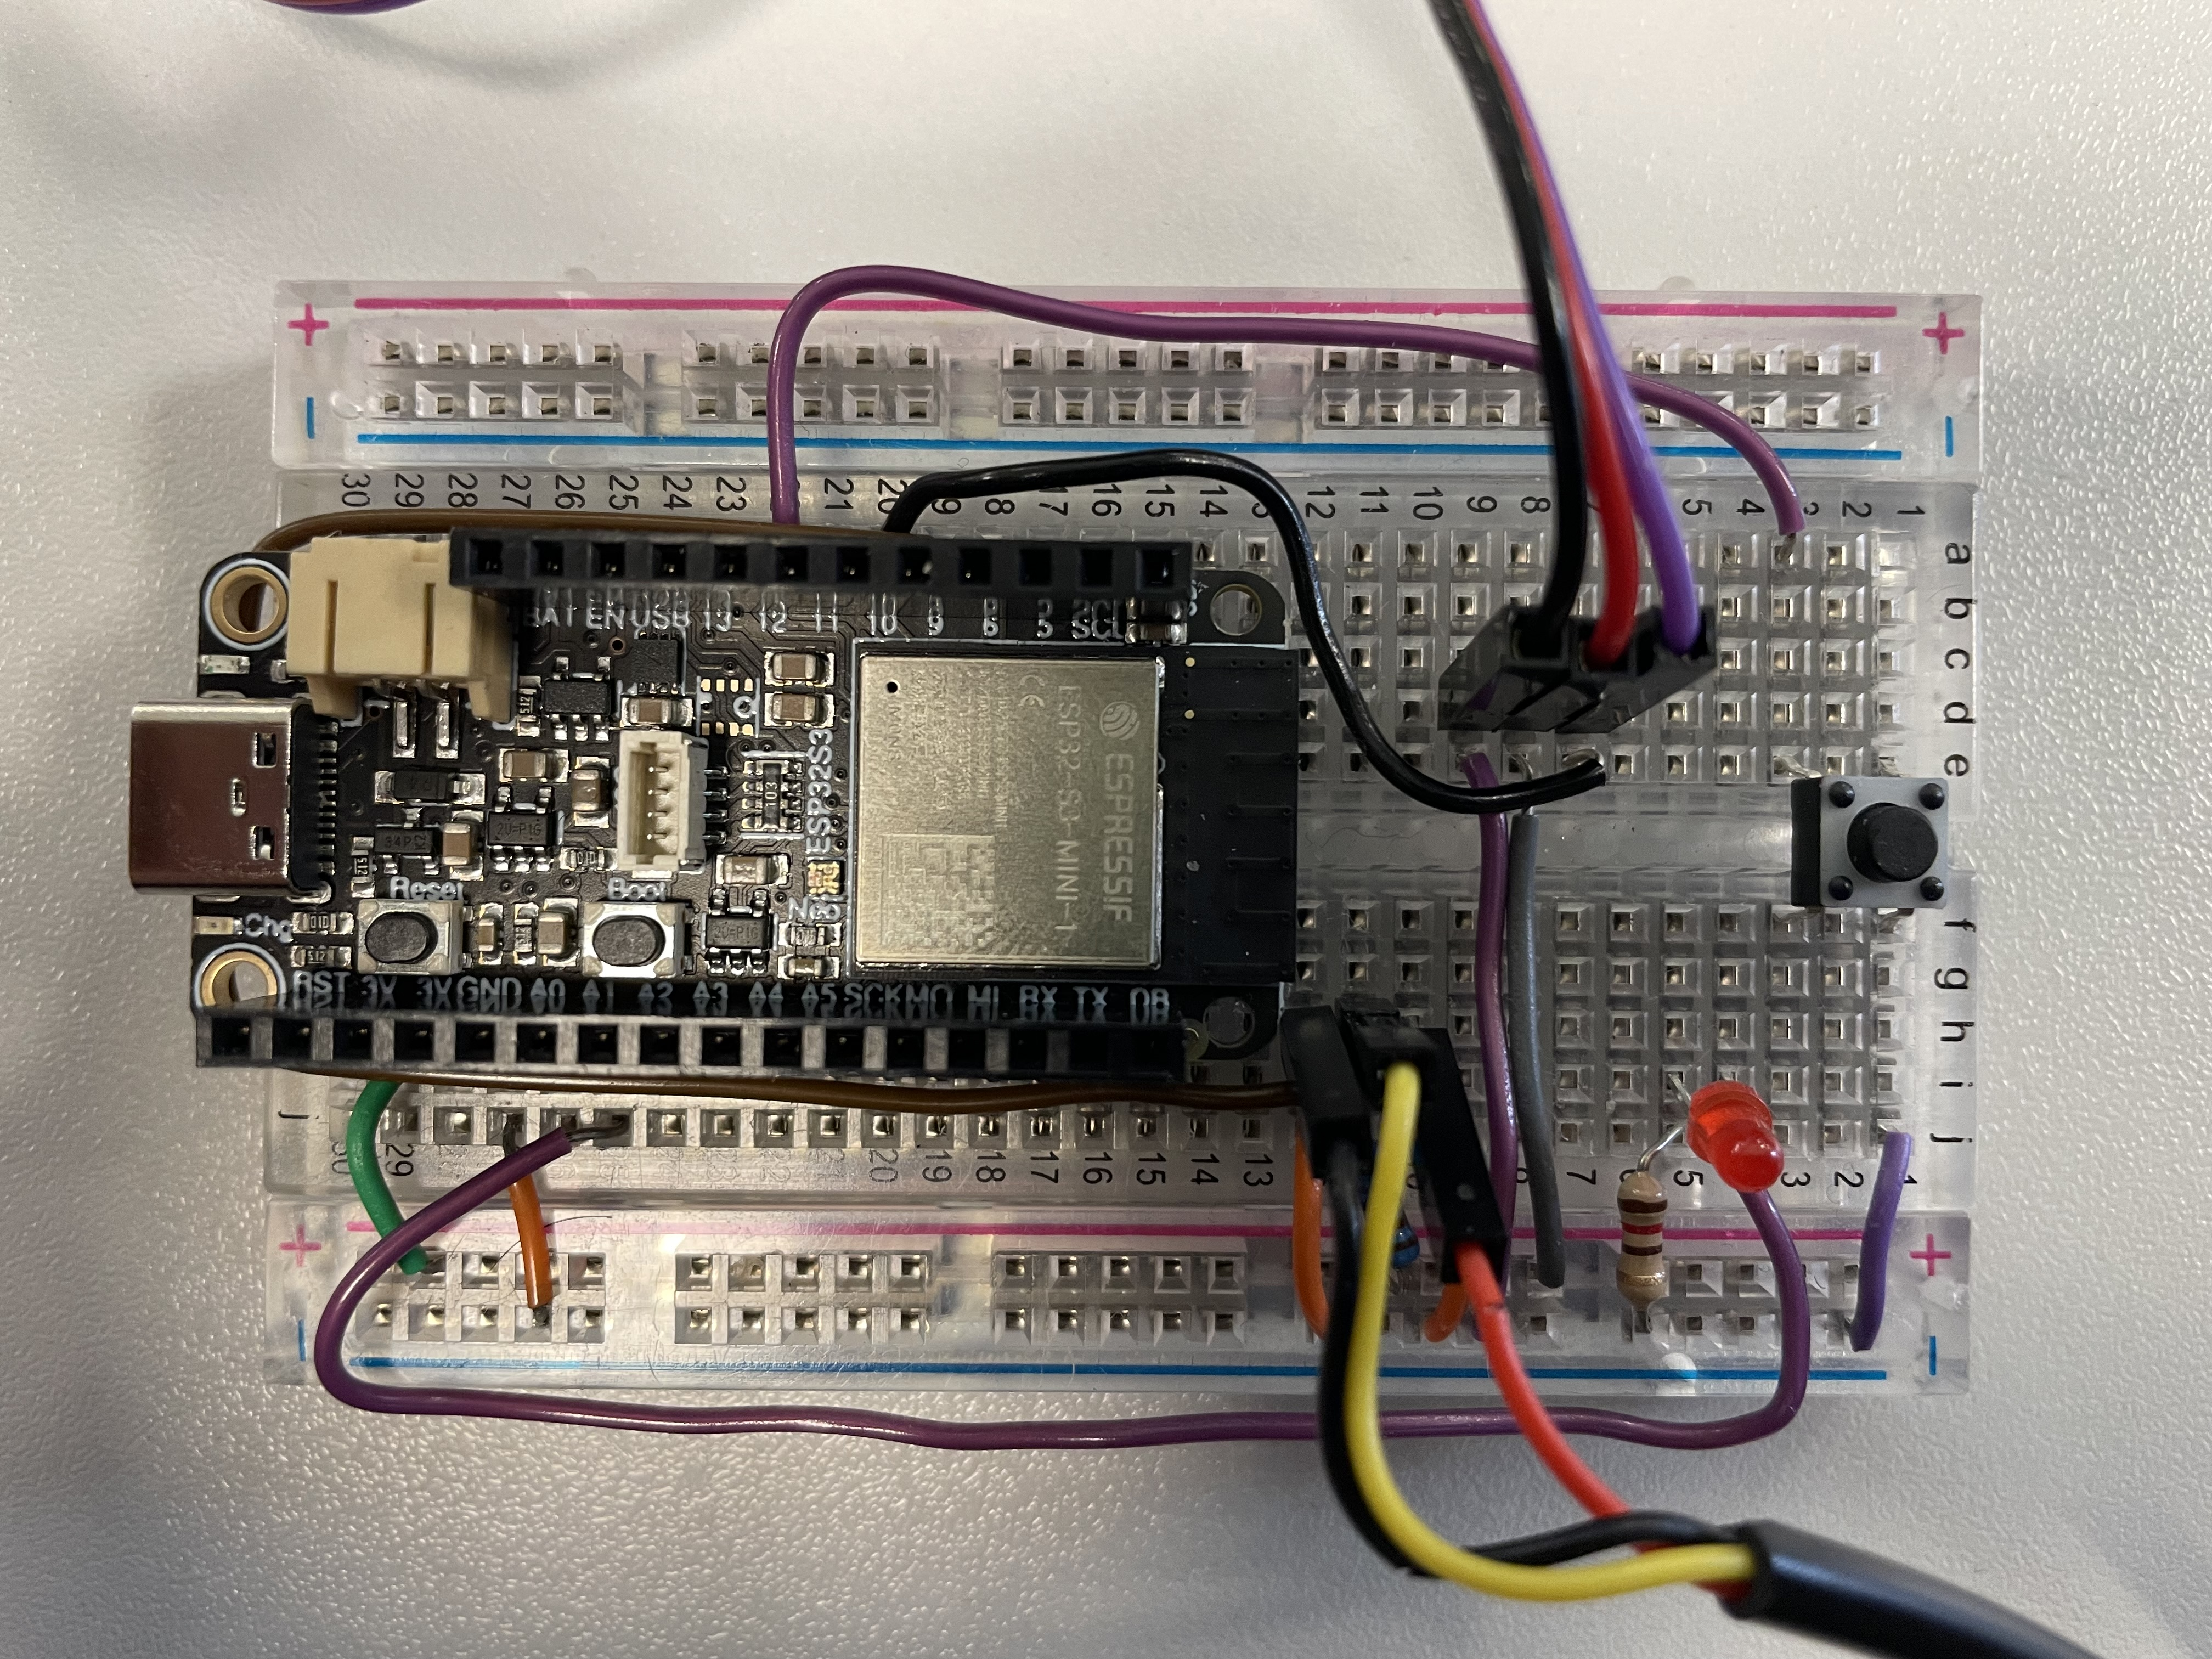
\includegraphics[width=\linewidth]{images/v6-hardware.jpg}
        \caption{Prototype}
        \label{fig:fig-proto}
    \end{subfigure}
    \hfill
    \begin{subfigure}[b]{0.45\linewidth}
        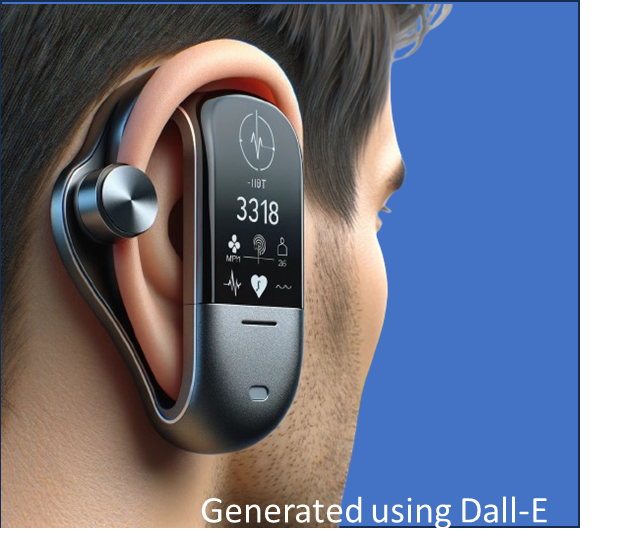
\includegraphics[width=\linewidth]{images/dall-e.png}
        \caption{Design Idea of Physical Product}
        \label{fig:fig-design}
    \end{subfigure}
    \caption{Smart Patch}
    \label{fig:fig-smartpatch}
\end{figure}

\section{Limitations and Issues Encountered}

\subsection{Trade off between Sensor Accuracy and Non-Intrusiveness}
In developing wearable devices for continuous monitoring, a significant challenge is balancing sensor accuracy with the need for non-intrusiveness, particularly for healthcare professionals (HCPs) who wear these devices during long shifts. High accuracy in sensors is crucial, as it ensures that the data collected is reliable enough to inform meaningful interventions to support HCP well-being. However, achieving this often requires more invasive technologies that may interfere with the daily activities and comfort of these professionals.\\ \\
VitalMonitor focuses on optimizing this balance by selecting sensors that minimize intrusiveness while still providing sufficiently accurate data for passive monitoring. This approach is critical in settings where both the well-being of HCPs and operational efficiency are prioritized. Given the limited availability of sensors that strike a perfect balance between non-intrusiveness and high accuracy, the selection was guided by the goal of maintaining user comfort and system reliability. This ensures that healthcare administrators can effectively monitor and respond to the health indicators of their staff without causing discomfort or disruption to their work.


\subsection{Converting Raw Data to Useful Data}

The DS18B20 Temperature Sensor and Pimoroni Pulse Sensor are integral to VitalMonitor's functionality, changing analog electrical signals into digital data for health monitoring. However, this reading process often introduces significant noise, resulting in irregular and unreliable data outputs.  Such anomalies, if unaddressed, could potentially trigger unwarranted alarms or actions based on incorrect information. This necessitates robust data processing strategies to ensure accuracy and usability. \\ \\
A common challenge in sensor data analysis is managing these irregularities, particularly when they lead to significant deviations from expected patterns. For example, an abrupt spike in temperature readings from 32 degrees Celsius to an erroneous 45 degrees could inadvertently exceed the system’s threshold of 35 degrees, resulting in false alarms. To ensure data integrity and reliability, it is imperative to employ robust data smoothing techniques. \\ \\
The Moving Average filter is one such technique applied within the VitalMonitor framework. By averaging data points over a defined time window, this method effectively dampens the impact of transient spikes or noise, leading to a more stable and accurate data output. This technique not only enhances the overall quality of the health monitoring data but also supports critical decision-making processes by reducing the likelihood of false alerts. Figure \ref{fig:data-sensors} provides a snapshot of data collected from the sensors in their raw form as well as data after implementing Moving Average function to it. \\

\begin{figure}[h!]
    \centering
    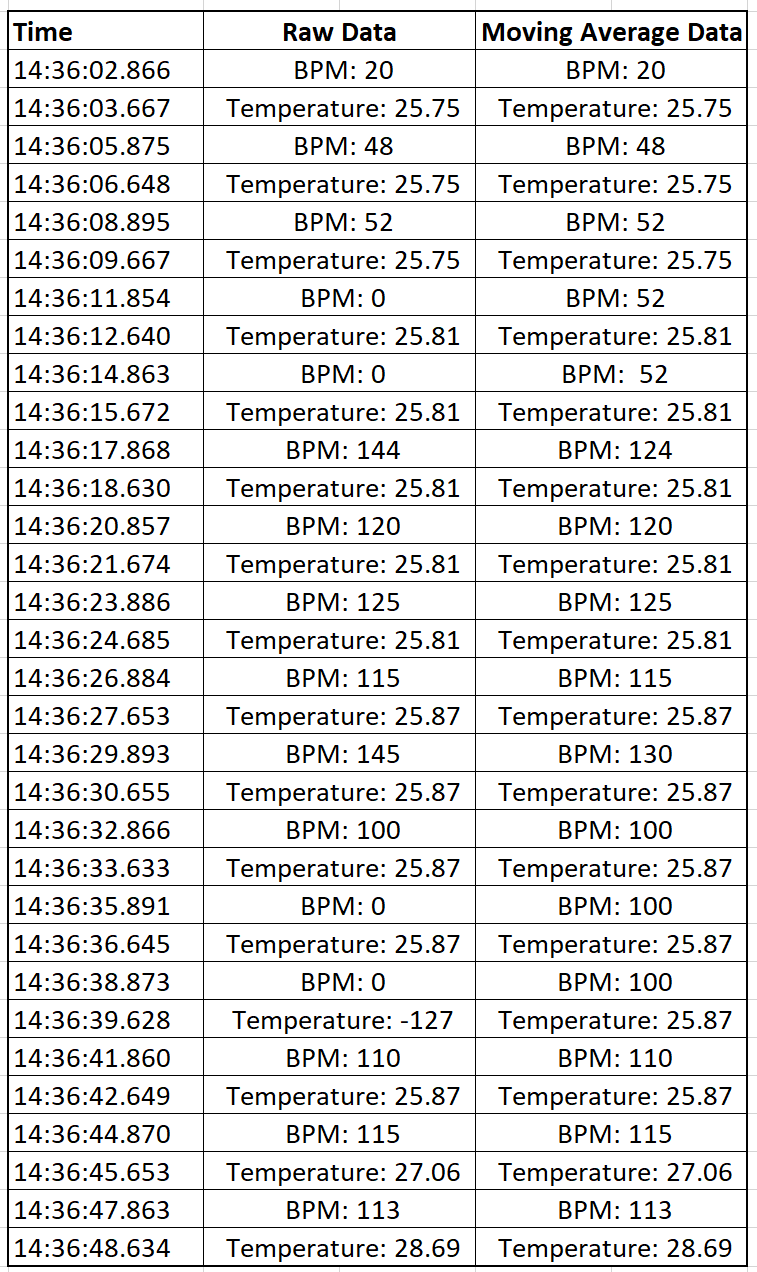
\includegraphics[width=0.6\linewidth]{images/data.png}
    \caption{Data from sensors}
    \label{fig:data-sensors}
\end{figure}

\noindent Extensive testing and evaluation have confirmed that the adapted sensors provide a data precision of \(\pm 15\) BPM for heart rate and \(\pm 0.2-0.5\) degree Celsius for temperature. These measures ensure that VitalMonitor delivers reliable and actionable health data for healthcare professionals, enhancing the monitoring and management of their well-being.

\subsection{Reliability depends on Network Bandwidth}
The effective operation of VitalMonitor’s Smart Patches heavily relies on the strength and capacity of the WiFi network to which they are connected. These devices are designed to upload data in real-time, a process that demands robust network performance to function seamlessly. With a scenario involving up to 100 Smart Patches transmitting data simultaneously, the bandwidth requirements become substantial. This substantial demand can strain the network, leading to potential data transmission delays that may impact the timeliness and reliability of data being displayed on the monitoring dashboard. \\ \\
During extensive testing and evaluation, it was observed that the system's reliability is significantly influenced by the WiFi network's bandwidth. Insufficient bandwidth can result in lagging data updates, which may hinder the system’s ability to provide real-time insights crucial for immediate decision-making and response. This finding underscores the necessity for implementing a network infrastructure capable of supporting high data loads, especially in environments where continuous and simultaneous monitoring is critical. Efforts to enhance network configurations, possibly through dedicated channels or enhanced WiFi protocols, are essential to mitigate these issues and ensure reliable system performance.

\subsection{Google Cloud}
Google Cloud offers \$300 in credits for database and server usage. In this project iteration, these credits were primarily utilized for the MySQL database, specifically the Enterprise Cloud SQL Edition. The chosen configuration, as depicted in Figure \ref{fig:cloud-configurations}, was optimized for cost efficiency, with an initial setup cost of \$6 and a daily operational cost of \$0.4. While suitable for development and testing purposes, this configuration may prove inadequate for production deployment, particularly when supporting a larger user base. \\

\begin{figure}[h!]
    \centering
    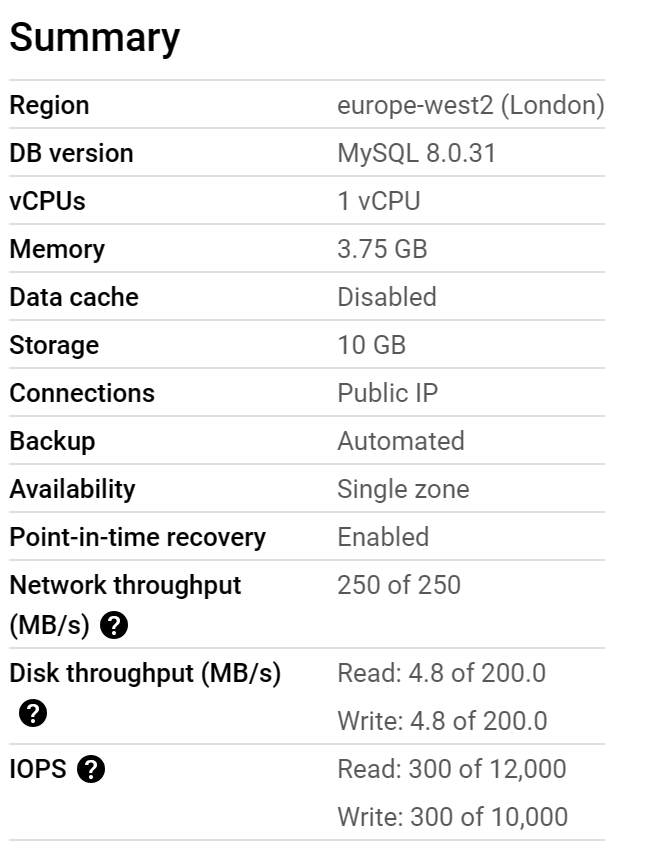
\includegraphics[width=0.5\linewidth]{images/cloud-configurations.png}
    \caption{Google Cloud Configurations}
    \label{fig:cloud-configurations}
\end{figure}

\noindent In a production environment scenario accommodating 100 HCPs and a single dashboard for hospital, upgrading database to the Enterprise Plus Cloud SQL Edition becomes imperative. This entails provisioning a minimum of 8 virtual CPUs, 32 GB of RAM, and increasing storage capacity to over 100 GB. Additionally, as the platform scales to serve multiple hospitals, resource requirements will escalate accordingly.\\

\noindent Furthermore, the middleware microservices will be deployed on Google Cloud in the production phase. These services interact with the database through HTTPS requests, utilizing unix-sockets with appropriate permissions. For instance, when an administrator adds a new device via the dashboard, the workflow involves traversing through the web page, web server, middleware, and database (hosted on Google Cloud) before returning. While deploying middleware on Google Cloud can streamline transactions and improve response times, it necessitates additional costs. Hence, this optimization was deferred in the current iteration to maintain cost-effectiveness.


\section{Further Work}
Despite having achieved the core objectives and beyond, there are more enhancements that this project could have done if not for the time constraint and knowledge-specific constraint. Further Work are divided into 3, things to be done to create a minimum viable product, improving current implementations and finally adding new requirements to make VitalMonitor more efficient.

\subsection{Smart Patch: Final Product}
The culmination of the Smart Patch project will yield a refined, compact device designed to discreetly rest behind the ear. This final iteration will feature optimized sensor placement, with the pulse sensor delicately positioned on the earlobe and the temperature sensor situated inconspicuously behind the ear. Transitioning from the current breadboard prototype to a fully soldered device with a 3D-printed cover will be pivotal, streamlining the product for mass production and enhancing its durability. A sample design was created for future device using Dall-E. This design is shown in Figure \ref{fig:fig-smartpatch}. Refer to Appendix \ref{chatgpt-prompts} for more information on how this image was generated. 

\noindent To achieve this, future efforts will focus on miniaturizing the device through advanced CAD design and employing more efficient microcontroller tailored specifically for the Smart Patch. However, before deployment, rigorous testing, including Electrical Safety Testing and Mechanical/Physical Testing, will be necessary to ensure compliance with industry standards and user safety. Although these tests were not feasible within the project's constraints, they remain critical future steps to validate the device's reliability and regulatory compliance.


\subsection{Improving the Middleware Infrastructure}
In future, the Middleware Infrastructure can be transitioned from a monolithic architecture to a more scalable and robust system comprising four distinct microservices. Currently, the infrastructure operates as a single web server, but the proposed evolution involves isolating functionality into four dedicated microservices: Session Management Service, User and Device Management Service, Data Ingestion Service, and Data Retrieval Service. By segmenting these services across different web servers, the workload is distributed more evenly, reducing the strain on any single server and enhancing system efficiency. \\ \\
This architectural enhancement not only fosters a clearer separation of concerns but also facilitates improved request management and scalability. Implementing a load balancer to orchestrate requests among these microservices ensures efficient data flow, minimizing the risk of data loss and optimizing overall system performance. This strategic restructuring lays the foundation for a more resilient and adaptable Middleware Infrastructure, poised to accommodate future growth and evolving user demands.

\subsection{Algorithm to Measure Stress and Fatigue Levels}
Existing methodologies lack a standardized approach to real-time measurement of stress and fatigue, primarily due to their multifaceted nature, influenced by a multitude of physiological and psychological factors. To address this challenge, further research is essential to develop an algorithm capable of quantifying these parameters quantitatively. This algorithmic approach aims to integrate various vital signs and personal information, providing a more comprehensive understanding of individual well-being beyond subjective descriptors like ``very stressed." Collaboration with medical researchers will be pivotal in discerning relevant parameters and assigning appropriate weights based on empirical evidence. By leveraging insights from medical literature and empirical data, the project will look in to refining decision-making processes and enhance the precision of stress and fatigue assessments. \\ \\
The ultimate goal is to streamline healthcare interventions and reduce reliance on simplistic thresholds, fostering a more nuanced approach to individual well-being monitoring. Although this entails extensive data gathering and analysis, its potential to expedite decision-making processes and improve healthcare outcomes underscores its significance in the realm of healthcare monitoring for HCPs.

\subsection{Interdisciplinary Collaboration for Enhanced Sensors}
Addressing the inherent trade-off between sensor accuracy and non-intrusiveness, it is neccessary to have interdisciplinary collaboration by electrical engineers and bio-medical engineers in this project. By pooling expertise from both fields, development of enhanced sensors will take place. These sensor(s) will be capable of accurately measuring vital signs such as heart rate and body temperature, while remaining non-intrusive to wear. This collaborative effort holds the potential to disrupt the healthcare industry by introducing innovative sensor technologies that prioritize both accuracy and user comfort.\\ \\
The development of non-intrusive sensors not only meets the demands of HCPs but also enhances the overall experience for patients undergoing medical treatments. By minimizing discomfort associated with traditional monitoring methods, non-intrusive sensors offer a more patient-centric approach to healthcare delivery, ultimately alleviating suffering and improving the quality of care. This interdisciplinary collaboration represents a pivotal step towards realizing the full potential of sensor technology in revolutionizing healthcare monitoring and patient outcomes.

\subsection{Prediction Model}
Stress and fatigue often rise gradually, with occasional spikes triggered by unforeseen events or stressors. Recognizing this pattern, future iterations will aim to develop a prediction model trained on actual human data. By forecasting stress levels before they surpass predetermined thresholds, this model provides early warning signals to healthcare organization administrators. Such anticipatory measures afford administrators more time to make necessary arrangements, mitigating the impact of heightened stress levels on healthcare professionals (HCPs) and optimizing patient care.\\\\
The integration of predictive analysis represents a notable advancement, augmenting VitalMonitor with cutting-edge AI and analytics functionalities. This strategic augmentation not only distinguishes the platform from competitors but also empowers healthcare organizations with foresight capabilities.